\section{Overview}
\label{sec:overview}
\begin{figure*}[t]
  \centering
  \begin{subfigure}[b]{0.4\textwidth}
  \centering
    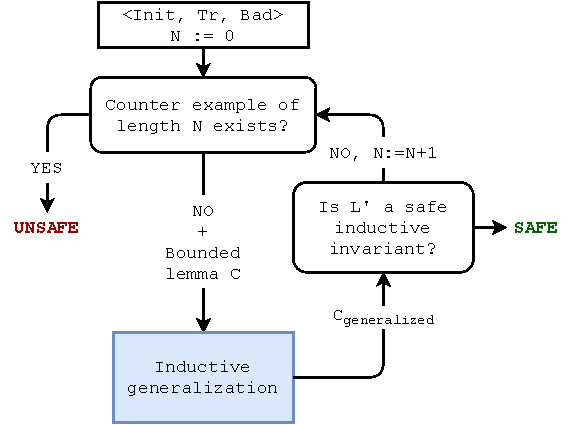
\includegraphics[height=4cm]{figures/doping-spacer}
    \caption{SMC architecture.}
    \label{fig:smc}
  \end{subfigure}
  \begin{subfigure}[b]{0.31\textwidth}
    \centering
    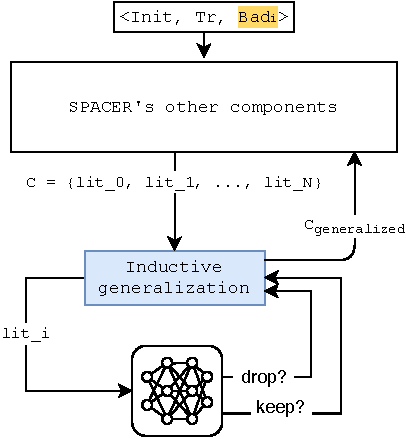
\includegraphics[height=4cm]{figures/doping-Page-general_architecture.pdf}
    \caption{\dpy architecture.}
    \label{fig:dopey}
	\end{subfigure}
  \begin{subfigure}[b]{0.15\textwidth}
  \centering
    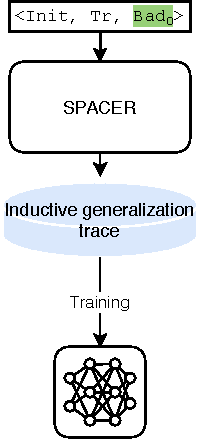
\includegraphics[height=4cm]{figures/doping-training.pdf}
    \caption{\dpy training.}
    \label{fig:spc_train}
	\end{subfigure}
	\caption{Overview of Symbolic Model Checking and overview of \dpy.}
  \label{fig:overview}
\end{figure*}
In this section, we give an overview of our technique, outline the challenges
involved, and our key insights to address them. The context is symbolic
SMT-based Model Checking (SMC)~\cite{IC3,GPDR,spacer}, also known as
satisfiability checking for Constrained Horn Clauses modulo Theory
(CHC)~\cite{DBLP:conf/birthday/BjornerGMR15}. In Model Checking, the high-level
goal is to show that an infinite state transition system ($Tr$) does not have an
execution/path that reaches a set of bad states ($\Bad$) by finding a formula
$\Inv$ that is an inductive invariant of $\Tr$ and does not intersect with
$\Bad$. The goal of CHC solving is to show that a set of First Order Logic
formulas $\Phi$ that satisfy the Horn
restriction~\cite{DBLP:conf/birthday/BjornerGMR15} is satisfiable by exhibiting
a symbolic formula $M$ that defines an FOL model that satisfies $\Phi$. The two
problems are closely related. Model Checking often reduced to CHC solving. Both
problems are in general undecidable.

\cref{fig:smc} shows the basic structure of an SMC algorithm based on IC3
architecture. In the paper, we use SMC \spc~\cite{spacer}, but the architecture is
common to many engines. SMC iteratively unrolls the $\Tr$, uses an SMT solver to
find a bounded counterexamples (which is usually decidable), and, if no
counterexample is found, attempts to create an inductive invariant. The
invariant is constructed as a set of so called \emph{lemmas}, where each lemma
is disjunction of atomic formulas. An example lemma is $x \leq 0 \lor y > 0$.
For convenience, we often represent lemmas as a set of formulas, writing instead
$\{x \leq 0,y > 0\}$. Many of the details of the algorithm are not important,
and we omit them here. The step we focus on in this paper is \emph{inductive
  generalization} (highlighted in blue in \cref{fig:smc}), that is responsible
for generalizing learned lemmas. In practice, this step is crucial for the
performance of SMC.

Conceptually, inductive generalization is a simple process, usually done with an
algorithm similar to the one we call \textsc{IterDrop}, shown in
\cref{alg:iter_drop}. \textsc{IterDrop} starts with a valid lemma $\ell = \{l_1,
\ldots, l_n\}$, and proceeds to generalize $\ell$ by removing an arbitrary
chosen literal from $\ell$, and using an SMT solver to check whether the lemma
is still valid (by calling \texttt{isInductive}). 
The details of \texttt{isInductive} are not important -- but it can be quite expensive. If the call succeeds, the literal is removed, otherwise it is kept. The goal is to generalize to a valid lemma with fewest literals.

From now on, when the context is clear, we use \emph{generalization} instead of inductive generalization.

% \setlength{\textfloatsep}{0pt}% Remove \textfloatsep
\begin{algorithm2e}[t]
\DontPrintSemicolon
\SetKwProg{Fn}{function}{}{end}

\SetKwFunction{Fdrop}{dropOne}
\SetKwFunction{Finductive}{isInductive}
\SetKwFunction{Fpick}{pick}


\KwIn{the original F-inductive lemma $L =\{l_1, l_2, ...,l_n\} $ }
\KwOut{a generalized F-inductive lemma $K \subseteq L $ }
$K \gets \emptyset $ \tcp*[l]{kept literals}  \label{line:spc-kept-lits}
$C \gets L $ \tcp*[l]{literals to check}

\While{$C \neq \emptyset  $}{
    $K,C \gets \Fdrop{K,C}$
}

\Return K
 
\vspace{4pt}

\Fn{\Fdrop{K, C}}{
    $lit \gets pick(C)$
    
    \uIf{ $\Finductive(K \cup\ C \setminus \{lit\})$} {
        $C \gets C \setminus \{lit\}$
    }
    \Else{
        $ K \gets K \cup \{lit\} $ ; %
        $C \gets C \setminus \{lit\}$
    }
    \Return $K, C$
}
\caption{\textsc{IterDrop} algorithm.}
\label{alg:iter_drop}
\end{algorithm2e}    

%%% Local Variables:
%%% mode: latex
%%% TeX-master: "../0.0_main"
%%% End:


We illustrate \textsc{IterDrop} with a sample run,  shown in
\cref{fig:spc_ind_gen}. \textsc{IterDrop} proceeds as follows:
\begin{itemize}
\item it tries to drop the first literal, $x_3 = \ltrue$, by checking whether
  $\ell'_1=\{x_1 = \ltrue, x_6 = 1, x_9 - x_{10} \geq 41, x_5 = 1\}$ is
  valid;
\item assume that $\ell'_1$ is valid, then $\ell \gets \ell'_1$, and $x_1 = \ltrue$ is chosen next;
\item now, assume that $\ell'_2 = \{x_6 = 1, x_9 - x_{10} \geq 41, x_5 = 1\}$ is
  not valid. $\ell$ remains as is and $x_6 = 1$ is chosen next;
\item assume that $\ell'_3 = \{ x_1 = \ltrue, x_9 - x_{10} \geq 41, x_5 = 1\}$ is valid, then
  $\ell \gets \ell'_3$, and $x_9 - x_{10} \geq 41$ is chosen next;
\item assume that $\ell'_4 = \{x_1 = \ltrue, x_5 = 1\}$ is not valid,
  then $\ell$ is unchanged, and $x_5 = 1$ is chosen next;
\item assume that $\ell'_5 = \{ x_1 = \ltrue, x_9 - x_{10} \geq 41\}$ is valid, then
  $\ell'_5$ is the final generalized lemma.
%   returned by \textsc{IterDrop}.
\end{itemize}
The example highlights the difficulty of inductive generalization. First, each
call to \texttt{checkInductive} is potentially very expensive. Thus, reducing
the number of the calls is highly desirable. Second, many of the calls, like
steps~2 and~4 are ``useless'' -- no new lemma is learned from them. Thus,
reducing such ``useless'' calls is also highly desirable. Finally, a solver
makes many (up to thousands) such inductive generalization calls per run.

\begin{figure*}[t]
    \centering
   \begin{subfigure}[b]{0.45\textwidth}
   \centering
        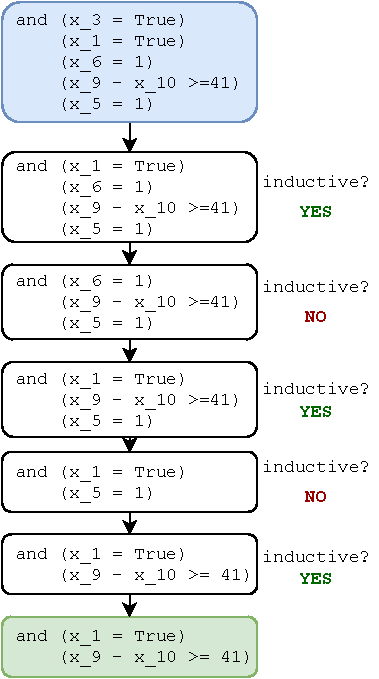
\includegraphics[width=0.8\textwidth]{figures/doping-spc_ind_gen.pdf}
        \caption{\textsc{IterDrop} example.}
    	\label{fig:spc_ind_gen}
	\end{subfigure}
    \begin{subfigure}[b]{0.45\textwidth}
    \centering
        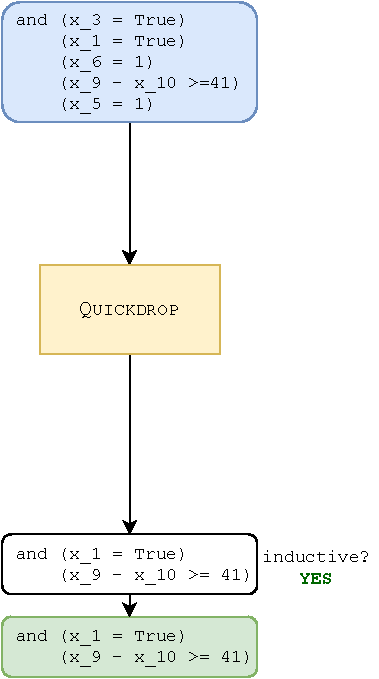
\includegraphics[width=0.8\textwidth]{figures/doping-spc_qd.pdf}
        \caption{\textsc{QuickDrop} example.}
    	\label{fig:spc_q_ind_gen}
	\end{subfigure}
	\caption{Examples of \textsc{IterDrop} and \textsc{QuickDrop}.}
    \label{fig:my_label}
\end{figure*}

\begin{figure*}[t]
    \centering
        \begin{subfigure}[b]{0.45\textwidth}
    \centering
        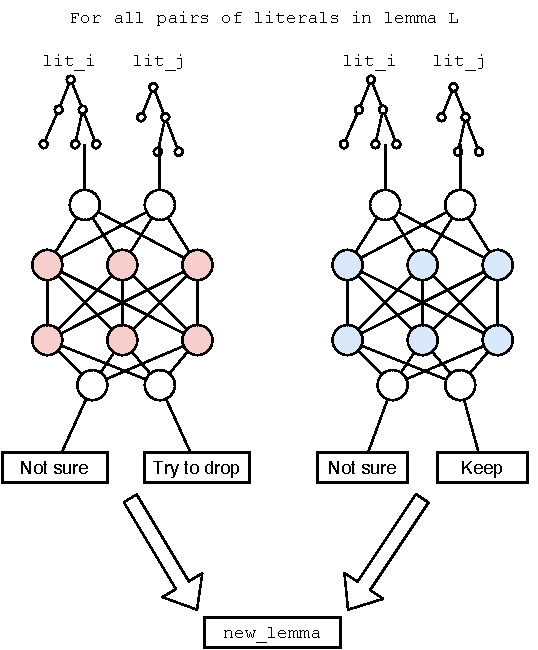
\includegraphics[width=0.8\textwidth]{figures/doping-model_vertical.pdf}
        \caption{\textsc{QuickDrop} example.}
    	\label{fig:spc_model_details}
	\end{subfigure}
	\begin{subfigure}[b]{0.45\textwidth}
	\centering
        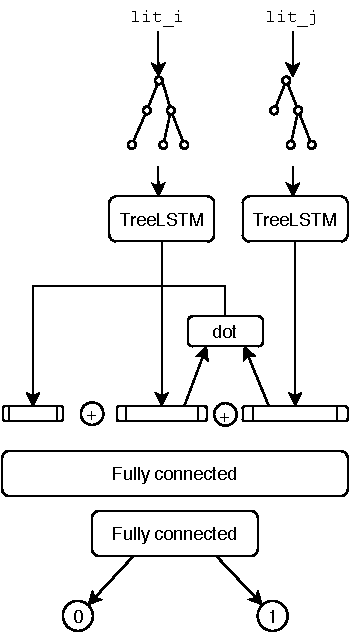
\includegraphics[width=0.6\textwidth]{figures/doping-model_detail.pdf}
        \caption{\textsc{QuickDrop} model.}
    	\label{subfig-4:model-detail}
	\end{subfigure}
    \caption{
      Architectures of \textsc{QuickDrop}.}
    \label{fig:architecture_of_qd}
\end{figure*}

Our \emph{key insight} is that since generalization happens
frequently, and, while the lemmas are different, the literals are similar, \emph{it is
possible to learn the co-occurrence between literals that do and do not occur in
the same lemma together}. We conjecture that once such a co-occurrence 
% (and anti-occurrence) 
is known, it can be used to guide \textsc{IterDrop} to make
fewer ``useless '' choices, and, ultimately, increase performance of SMC.
Furthermore, to avoid the difficulties of online learning, we rely on the fact
that many systems come with multiple properties (i.e., $\Bad$ states), and
learning from solving one property can be transferred to solving another.

Concretely, we propose a new SMC, called \dpy. As shown in
\cref{fig:dopey}, \dpy combines symbolic reasoning with guidance by a
neural network. The core of \dpy is a new neural-based generalization
algorithm called \textsc{QuickDrop}. Its pseudo-code is shown
in~\cref{alg:qdrop}. \textsc{QuickDrop} uses two neural networks, denoted by
$\Mpos$ and $\Mneg$, to predict whether a currently
chosen literal should be kept in the lemma or dropped. The prediction is based on past co- and anti-occurrences of pairs of  literals in lemmas. 

%Detailed description of \textsc{QuickDrop} is given in
%\cref{alg:qdrop}.

We illustrate a run of \textsc{QuickDrop} on the same example as
\textsc{IterDrop}. Recall that the initial lemma is $\ell = \{x_3 =
\ltrue, x_1 = \ltrue, x_6 = 1, x_9 - x_{10} \geq 41, x_5 = 1\}$.
% \ag{At this point, I do not understand the example. Please update it to be similar to the example for \textsc{IterDrop}.}
Assume that $x_1 = \ltrue$ is checked and kept, \tool proceeds as follows:
\begin{itemize}
\item it runs $\Mpos$ and predicts that $\{x_9 - x_{10} \geq 41\}$ should be kept;
\item it runs $\Mneg$ and predicts that $\{x_3 =
\ltrue, x_6 = 1\}$ should be dropped;
\item it combines the results from steps~1 and~2 and suggests a candidate $\ell_{cand}=\{x_1 =
  \ltrue, x_9 - x_{10} \geq 41\}$;
\item it checks the inductiveness of $\ell_{cand}$.
\end{itemize}
Note that \tool runs only \emph{one} inductiveness
check, compared to 5 used by \textsc{IterDrop}.
% (\cref{fig:spc_ind_gen}).

% \ag{I assume that example ends here}

% Given a lemma $\ell$, \dpy uses a neural component
% to predict which literals should be dropped and kept.


% \cref{fig:spc_train} shows how to train such component: we simply runs \spc to
% verify $\trs$, record the traces to a dataset, and use the dataset to train the
% neural component.

The key idea of \textsc{QuickDrop} is to use the \textit{co-occurrence} and
\textit{anti-occurrence} between literals in lemmas to predict which literals are
likely to be together in future lemmas. This intuition comes from an
observation that in many generalizations either: (a) a literal is
always got removed whenever another literal is kept (anti-occurrence) or (b) a
literal is kept whenever another literal is also kept (co-occurrence). We believe
that a) happens because the state space of a typical system under analysis can
be partitioned into disjoint components, and many lemmas reference only a few of
the components at a time; and b) happens because those literals are part of the same piece-wise linear function.

To learn the desired anti- and co-occurrence, we use two neural networks, called
$\Mneg$ and $\Mpos$, respectively. The networks are trained based on a run of an
SMC on a problem instance. We gather the set of all lemmas and their
generalizations, and use the data to train the network. Each network predicts,
given a literal $l_i$ the likelihood that a literal $l_j$ appears in a lemma
together with $l_i$. The details of the training are given in \cref{sec:learning-signal}.


% could be separated into disjoint areas, thus literals over variables
% in one area should be drop in a lemma over variables in a different area
% (antirelation). On the other hand, literals those together form a piecewise
% linear function that is used over and over should always stay together, since
% they are in fact parts of the same function (correlation). \ag{Parts of this
%   paragraph need to migrate to the insight above.}


%   \cref{fig:spc_train} shows how to train such component: we simply runs \spc to
%   verify $\trs$, record the traces to a dataset, and use the dataset to train the
%   neural component.

% \ag{This paragraph does not work. It is way too detailed for the overview.}
% \textsc{QuickDrop} uses two separated neural networks $\Ppos$ and $\Pneg$ (shown
% in blue and red, respectively, in \cref{subfig-4:model}). Given a pair of
% literals $(l_i, l_j)$ such that $l_i$ is already kept, $\Pneg$ predicts whether
% $l_j$ should be dropped, and $\Ppos$ predicts whether it should be kept. The
% details are shown in \cref{alg:qdrop}, where the blue lines mark the key
% differences between \textsc{IterDrop} and \textsc{QuickDrop}. Instead of 
% checking one literal at a time, \textsc{QuickDrop} predicts whether to drop or keep a set of
% literals (lines 4--5). We also need to \textsc{seed} the 2 networks by calling
% line 1 to keep at least a literal.  Let's see how
% \tool works on the same example as \textsc{IterDrop}.

\paragraph{Challenges.}
To make \dpy a practical verification engine, we have to address challenges in
three aspects: (a) machine learning, (b) logical soundness, and (c) engineering. For
machine learning, the challenge is in representing symbolic expressions as
vectors, while maintaining their rich semantic structure to enable to learn and
generalize co-occurrences between them. For logical soundness, the challenge is to use the neural nets
in a way that guarantees the soundness of a verification engine.
For engineering, the challenge is to
integrate ML and symbolic components in an effective way.

\paragraph{Representation learning of symbolic formula.}
Unlike raw images or natural language text, for which there are standard deep
learning models including convolutional and recurrent neural networks, a literal
in a lemma is a symbolic formula, which is structured and meaning of which is
sensitive to small changes. Simply viewing a literal as a sequence of tokens, as
in NLP, fails to capture the subtle semantic differences between structurally
similar literals.
    
    
We incorporate both syntactic and semantic information of a literal into its
representation. Our approach views a literal as a directed acyclic graph (DAG),
which is post-processed from its abstract syntax tree (AST), and
then adapts TreeLSTM~\cite{TreeLSTM} to embed such a DAG structure. Our approach
also takes semantic level information into consideration so that specific
properties of values are respected. For instance, embedding of numerical
values should preserve their relative order and equality.
    

% AG: someone, please move to macros
\begin{figure}[t]
  \centering
  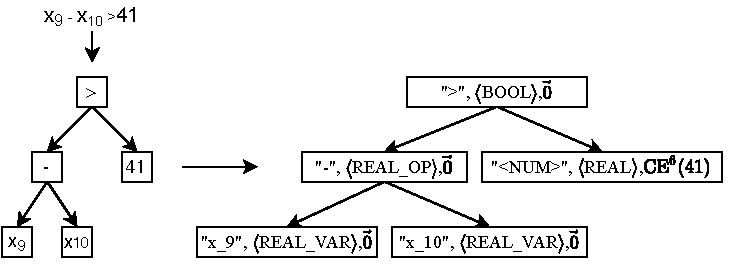
\includegraphics[width=0.8\textwidth]{figures/doping-ast-exp.pdf}
  \caption{An example of an AST and its semantic features.}
  \label{fig:ast_example}
\end{figure}

%%% Local Variables:
%%% mode: latex
%%% TeX-master: "0.0_main"
%%% End:


\paragraph{Learning for inductive generalization.}
Directly using machine learning to address the generalization problem
is a non-trivial structure prediction problem. It takes in a set of symbolic
formulas and outputs another set of symbolic formulas that are more
general and more concise. Though in principle, sequence-to-sequence
models~\cite{lample2019deep} are applicable, they are unlikely to accomplish such a
complicated reasoning task with existing ML models. In fact, even predicting
equivalence between two simple symbolic expressions remains
challenging~\cite{Allamanis:icml17}. Rather than having an end-to-end ML
solution, we embed a learning component in a classic symbolic approach of
generalization. Specifically, the learning component captures the
co-occurrence between literals appearing in past runs and predicts the likelihood
of keeping or dropping a literal in the current run.
Furthermore, uncertainties introduced by the learning component 
have to be carefully controlled, which otherwise could lead to
unsound conclusion. \dpy is designed to make sound progress no 
matter what predictions the learning component provides. Bad
predictions may be harmful to the performance, but not to soundness! 
   
    
\paragraph{Integrating machine learning with logical reasoning.}
ML models and logical reasoning framework are implemented in very different
programming environments and rely on different hardware. Their
integration unavoidably involves communication overhead among different runtimes and
hardware. This may offset performance gains of fast prediction, posing a significant engineering challenge. 
%
%Furthermore, uncertainties introduced by the learning component 
%have to be carefully controlled, which otherwise could lead to
%unsound conclusion. \dpy is designed to make sound progress no 
%matter what predictions the learning component provides. Bad
%predictions may be harmful to the performance, but not to soundness! 

% In particular, \dpy uses a positive model and a negative model
% at the same time to achieve more reliable predictions.

% \paragraph{Evaluation of neuro-symbolic design.}
% A straightforward way of evaluating a new design is to measure the run time used
% on solving some instances. The shorter, the better. However, the intricate
% complexity of a logical reasoning framework like \spc makes such a simple
% measurement problematic. A random decision at a particular step leads the
% subsequent search or reasoning to a very different direction, which may boost
% the performance accidentally. On the other hand, longer run time does not
% necessarily indicate that the learning component has no or negative value.
% Because the performance gain of having a learning (or neuro) component can be
% counteracted by two factors: the subsequent actions assuring soundness, and the
% communication overhead between the neuro part and the symbolic part. Our
% evaluation first analyzes the effectiveness of the learning component with a
% number of different design choices in various application scenarios, and then
% measures the gain or overhead of each component in wallclock time and other
% metrics like number of queries and number of inductive generation iterations.
% \ag{I don't think current evaluation section address the issues in this
%   paragraph. If we do not address these issues, we should move it into
%   discussion after experimental results. Say that we only measure run time, but
%   that is not necessarily adequate and one of the limitations to address in the
%   future.}\NL{I agree. Also I prefer 3 challenges over 4 anw}
%%% Local Variables:
%%% mode: latex
%%% TeX-master: "0.0_main"
%%% End:
